\section{Giới thiệu}\label{sec:intro}
\frame{\tableofcontents[currentsection]}
\begin{frame}{Giới thiệu}

\begin{itemize}
    \item Là một bài toán tạo sinh dữ liệu dạng hình ảnh dựa trên các dạng dữ liệu khác.
    \item Cho trước một vài dữ liệu về gương mặt của một người bất kỳ \textit{(hình ảnh, video ngắn)} và môt đoạn tiếng nói bất kỳ. Tạo sinh hình ảnh người đó đang nói đoạn tiếng nói đã cho một cách chân thực.
\begin{figure}[H]
    \centering
    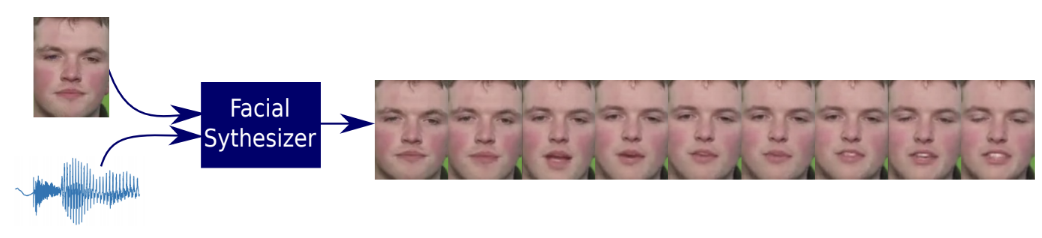
\includegraphics[width=13cm]{images/intro.png}
    \caption{Ví dụ về mô hình tạo sinh khuôn mặt}
    \label{fig:example}
\end{figure}
\end{itemize}
\end{frame}
